 

\section*{Problem 1}
	\begin{enumerate}[(a)]
	\item
		Computer aided design (CAD) is the practice of using computers to assist in 
		the creation and modification of designs.
		
	\item
		A printed circuit board (PCB) is a thin plate on which electronic components 		
		are placed.
		
	\item
		A programmable logic board (PLD) is a chip with generic architecture and a 
		collection of programmable switches, allowing the designer to match the chip 
		to the desired functionality.
		
	\item
		A field-programmable gate array (FPGA) contains billions of transistors and can 
		implement complex digital systems.
		
	\end{enumerate}
		
\section*{Problem 2}
	\begin{enumerate}[(a)]
	\item 
		In terms of time, the design-simulation-verification is more expensive because modern CAD programs have become extremely sophisticated, to the point that design problems that would be discovered in the implementation-testing-verification loop are caught and dealt with before a prototype is ever made. This means that the design work is increasingly moving from the real world to the computer.
		
		In terms of money, the answer depends on what is being designed. If it is something made with cheap materials, such as a plastic cup, then the cost of the time it took the engineer to design the cup is more expensive than the cost of every cup ever designed. As the materials/manufacturing become more expensive, however, the cost of implementing the design eventually outweighs the time of the engineer who designed it.
		
		\item The implementation-testing-verification loop can be skipped, and often is in the case of extremely large designs such as skyscrapers or dams where it is unfeasible to build a prototype. The penalty for doing this is the risk of a failure that a computer can't simulate, but this penalty is becoming less onerous as CAD technology progresses.

	\end{enumerate}


\section*{Problem 3}
	\begin{enumerate}[(a)]
		\item $ 1* 2^0 + 1 * 2^ 3 + 1* 2^5 + 1* 2^6 =105$
		\item $ 1* 2^0 + 1 * 2^2 + 1 * 2^3 = 13$
		\item $1* 8^ 0 + 1* 8 ^ 2 + 1 * 8^3 =577$
		\item $ 1* 16^0 + 1* 16^ 2 + 1* 16^ 3 = 4353$
		
	\end{enumerate}

\section*{Problem 4}
When not specified, a number's base is 10.

	\begin{enumerate}[(a)]
		\item $45 = 32 + 8 + 4 + 1 = 2^5 + 2^ 3 = 2^2 + 2^0 = 101101_2$
		\item $281= 256 + 16 + 8 + 1 = 2^8 + 2 ^ 4 + 2^ 3 + 2 ^0 = 100011001_2$
		\item $281_{16} = 2*16^2 + 8*16^1 + 1 * 16^0 = 641$
		
				$641 = 512 + 128 + 1 = 2^9 + 2^7 + 2^0 = 1010000001_2$

		\item  $CAD_{16} = 12* 16^2 + 10 * 16^1 + 13* 16^0 = 3245$
					\begin{align*}
					3245 / 2 &= 1622 &\bmod 1\\
					1622 /2 &= 811 &\bmod 0\\
					811 /2 &= 405 &\bmod 1\\
					405 /2 &= 202 &\bmod 1\\
					202 /2 &= 101 &\bmod 0\\
					101 /2 &= 50 &\bmod 1\\
					50 /2 &= 25 &\bmod 0\\
					25/2 &= 12 &\bmod 1\\
					12/2 &= 6 &\bmod 0\\
					6/2 &= 3 &\bmod 0\\
					3/2 &= 1 &\bmod 1\\
					1/2 &= 0 &\bmod 1
					\end{align*}
					
				Reading the remainders from most significant to least significant (bottom to top), we find that $CAD_{16} = 110010101101_2$.

		
	\end{enumerate}

\section*{Problem 5}
	To see the movie, you must satisfy one of four scenarios:
	
	\begin{itemize}
		\item A = 1, S = 0, with any combination of the other variables
		\item B = 1, S  =0, with any combination of the other variables
		\item A = 1, T1 = 1, with any combination of the other variables
		\item B = 1, T2 = 1, with any combination of the other variables
	\end{itemize}
	

\section*{Problem 6}
	\begin{enumerate}[(a)]
	
	\item \adjustbox{valign=t}{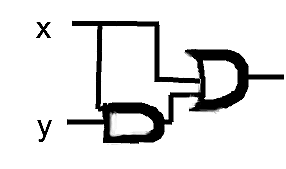
\includegraphics[scale=.5]{xy.png}}
	\item
	\begin{displaymath}
	\begin{array}{|c|c|c|c}
	x
	& y
	& xy
	& x + xy \\
	\hline
	0 & 0 & 0 & 0 \\
	0 & 1 & 0 & 0 \\
	1 & 0 & 0 & 1 \\
	1 & 1 & 1 & 1 \\	
	\hline
	\end{array}
	\end{displaymath}		
	
	\item An equivalent expression is $f(x,\, y) = x$
	\end{enumerate}

\section*{Problem 7}
	\begin{enumerate}[(a)]
		\item F = \={A}BC + \={A}B\={C} + AC
		\item 
		\begin{displaymath}
		\begin{array}{|c|c|c|c|c|c|c}
		A
		& B
		& C 
		& \overline{A}BC
		& \overline{A}B\overline{C}
		& AC
		& F = \overline{A}BC + \overline{A}B\overline{C} + AC \\
		\hline
		0 & 0 & 0 & 0 & 0 & 0 & 0 \\
		0 & 0 & 1 & 0 & 0 & 0 & 0 \\
		0 & 1 & 0 & 0 & 1 & 0 & 1 \\
		0 & 1 & 1 & 1 & 0 & 0 & 1 \\
		1 & 0 & 0 & 0 & 0 & 0 & 0 \\
		1 & 0 & 1 & 0 & 0 & 1 & 1 \\
		1 & 1 & 0 & 0 & 0 & 0 & 0 \\
		1 & 1 & 1 & 0 & 0 & 1 & 1 \\
		\hline
		
		
		\end{array}
		\end{displaymath}
		
	\end{enumerate}


\end{document}